%\documentclass[a4paper]{article}
%\usepackage{geometry}
%\geometry{a4paper,scale=0.8}
\documentclass[8pt]{article}
\usepackage{ctex}  % 支持中文
\usepackage{indentfirst}  % 首行缩进
\usepackage{longtable}  % 支持长表格
\usepackage{multirow}  % 支持多行单元格
\usepackage[a4paper, 
top=1in, bottom=1in, left=0.8in, right=0.8in,
]{geometry}  % 设置页面尺寸和边距
\usepackage{CJK}  % 支持中文
\usepackage[fleqn]{amsmath}
\usepackage{parskip}
\usepackage{listings}
\usepackage{fancyhdr}
\usepackage{hyperref}
\pagestyle{fancy}

% 设置页眉
\fancyhead[L]{2024年秋季}
\fancyhead[C]{机器学习}
\fancyhead[R]{作业二}


\usepackage{graphicx}
\usepackage{float}
\usepackage{multicol}
\usepackage{amssymb}
\usepackage{booktabs}
\usepackage{xcolor}

% 定义Python代码风格
\definecolor{codegreen}{rgb}{0,0.6,0}
\definecolor{codegray}{rgb}{0.5,0.5,0.5}
\definecolor{codepurple}{rgb}{0.58,0,0.82}
\definecolor{backcolour}{rgb}{0.95,0.95,0.92}

\lstdefinestyle{mystyle}{
    backgroundcolor=\color{backcolour},   
    commentstyle=\color{codegreen},
    keywordstyle=\color{magenta},
    numberstyle=\tiny\color{codegray},
    stringstyle=\color{codepurple},
    basicstyle=\ttfamily\footnotesize,
    breakatwhitespace=false,         
    breaklines=true,     
    captionpos=b,        
    keepspaces=true,     
    numbers=left,        
    numbersep=5pt,       
    showspaces=false,    showstringspaces=false,
    showtabs=false,      
    tabsize=2
}

\lstset{style=mystyle}
\begin{document}

\textbf{\color{blue} \Large 姓名:毛九弢 \ \ \ 学号:221900175 \ \ \ \today}

\section*{零. 实验环境}
\begin{itemize}
    \item 操作系统:Windows 11
    \item Python 版本:3.9.19
    \item 依赖库:见requirements.txt
\end{itemize}

\section*{一. (30 points) 类别不平衡 [本题题面对正负样本的描述描述反了]}

信用卡欺诈检测数据集 (Credit Card Fraud Detection)包含了2013年9月通过信用卡进行的欧洲持卡人的交易。这是一个非常典型的类别不平衡数据集,数据集中正常交易的标签远多于欺诈交易。请你根据附件中提供的该数据集完成以下问题:

参考链接: 
\url{https://zhuanlan.zhihu.com/p/134091240},
\url{https://scikit-learn.org/stable/modules/generated/sklearn.svm.SVC.html#sklearn.svm.SVC},
\url{https://www.cnblogs.com/linjingyg/p/15708635.html}.

\subsection*{代码说明}
\begin{itemize}
    \item 代码见压缩包code中的Prob1, 代码详细说明见Prob1中的README文件; 
    \item 详细输出见Prob1中的out文件夹。
\end{itemize}

\subsection*{Task1}
该数据集共有284807个样本,其中只有492个负样本。请按照训练集和测试集比例4:1的方式划分数据集(使用固定的随机种子)。在训练集上训练SVM模型,并计算该模型在测试集上的精度(如准确率、召回率、F1分数,AUC等)。请展示SVM模型训练过程的完整代码,并绘制ROC曲线(8 points);

\begin{minipage}{\textwidth}
    \begin{minipage}{0.65\textwidth}
        \begin{table}[H]
            \caption{SVM模型性能}
            \raggedright
            \begin{tabular}{cccccc}
            \toprule
            指标 & ACC & PRE & REC & F1 & AUC \\
            \midrule
            SVM & 0.999350 & 0.906667 & 0.693878 & 0.786127 & 0.968045\\
            \bottomrule
            \end{tabular}
        \end{table}
    \end{minipage}
    \begin{minipage}{0.35\textwidth}
        \begin{figure}[H]
            \raggedright
            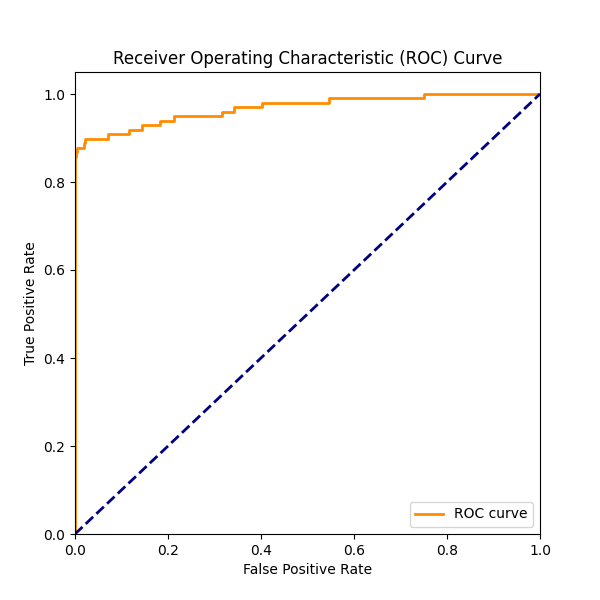
\includegraphics[width=\textwidth]{../Prob1/out/rand_seed_14/task1/roc_curve.png}
            \caption{ROC曲线}
        \end{figure}
    \end{minipage}
\end{minipage}
\subsection*{Task2}
请从上述训练集中的正样本中分别随机剔除2000,20000,200000个样本,剩余的正样本和训练集中原本的负样本共同组成新的训练集,测试集保持不变。请参照上一小问方式在这三个新的训练集上训练svm模型,并记录每个模型的精度。观察并比较这几组实验的结果,结合准确率与召回率的定义,请说明不平衡数据集对模型的影响(9 points);
\subsection*{2.1 结果}
\begin{table}[H]
    \centering
    \caption{剔除不同数目样本的SVM模型性能}
    \begin{tabular}{cccccc}
    \toprule
    指标 & ACC & PRE & REC & F1 & AUC \\
    \midrule
    SVM & 0.999350 & 0.906667 & 0.693878 & 0.786127 & 0.968045\\
    \midrule
    SVM-2k & 0.999350 & 0.906667 & 0.693878 & 0.786127 & 0.968553\\
    \midrule
    SVM-2w & 0.999368 & 0.907895 & 0.704082 & 0.793103 & 0.969577\\
    \midrule
    SVM-20w & 0.999298 & 0.802083 & 0.785714 & 0.793814 & 0.973112\\
    \bottomrule
    \end{tabular}
\end{table}
\begin{figure}[H]
    \centering
    \begin{minipage}{0.7\textwidth}
        \centering
        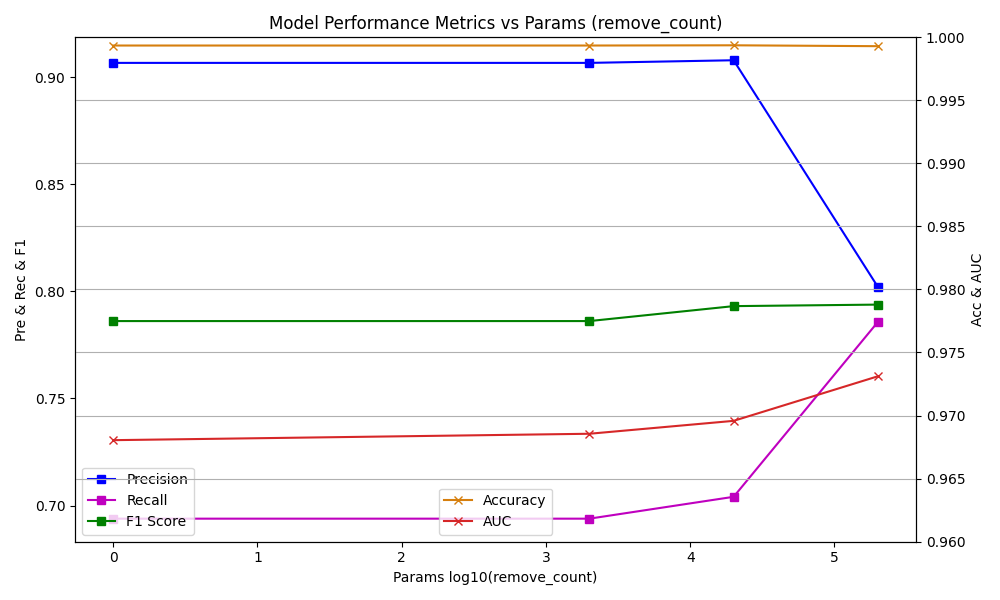
\includegraphics[width=\textwidth]{../Prob1/out/rand_seed_14/task2/Metrics_curve_rc_0_2k_2w_20w.png}
        \label{fig:Metrics_curve_rc_0_2k_2w_20w}
        \caption{变化曲线}
    \end{minipage}
\end{figure}
剔除不同数目样本的ROC曲线
\begin{figure}[H]
    \centering
    \begin{minipage}{0.32\textwidth}
        \centering
        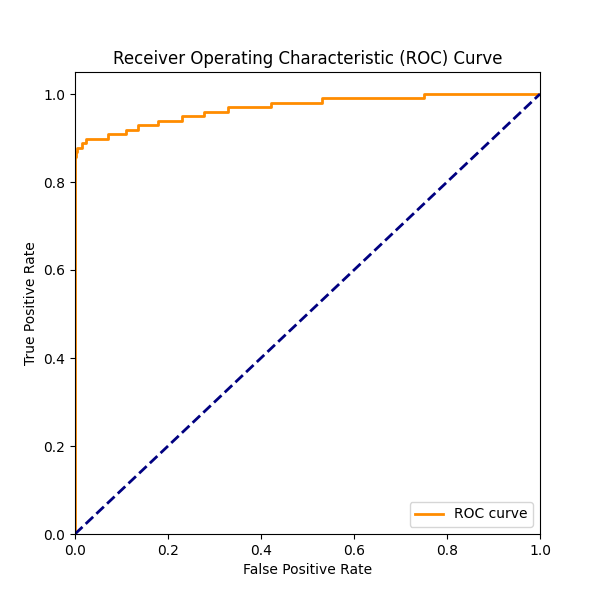
\includegraphics[width=\textwidth]{../Prob1/out/rand_seed_14/task2/roc_curve_remove2000.png}
        \caption{剔除2000个样本}
        \label{fig:roc_curve_remove2000}
    \end{minipage}
    \hfill
    \begin{minipage}{0.32\textwidth}
        \centering
        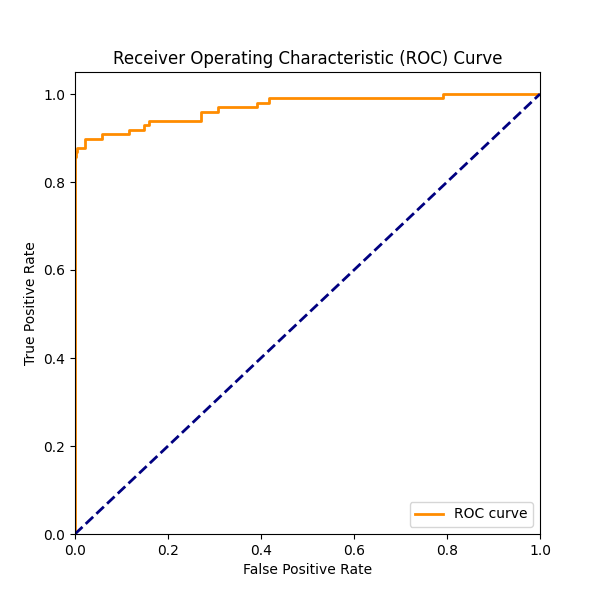
\includegraphics[width=\textwidth]{../Prob1/out/rand_seed_14/task2/roc_curve_remove20000.png}
        \caption{剔除20000个样本}
        \label{fig:roc_curve_remove20000}
    \end{minipage}
    \hfill
    \begin{minipage}{0.32\textwidth}
        \centering
        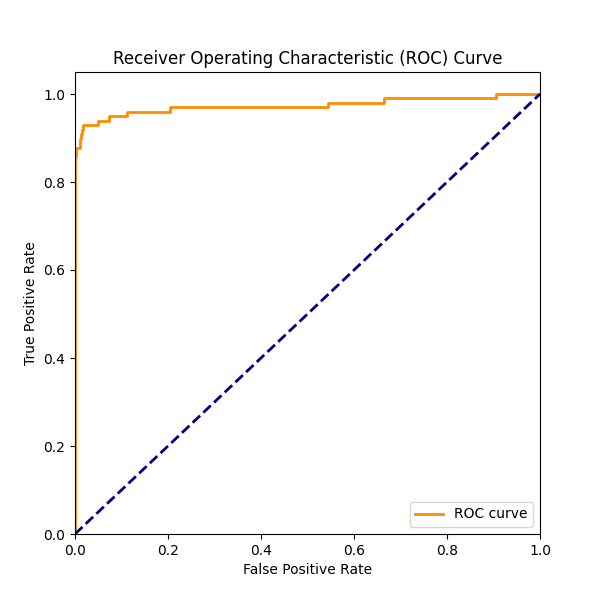
\includegraphics[width=\textwidth]{../Prob1/out/rand_seed_14/task2/roc_curve_remove200000.png}
        \caption{剔除200000个样本}
        \label{fig:roc_curve_remove200000}
    \end{minipage}
    \hfill
\end{figure}

\subsection*{2.2 结论}

PRE 和 REC 的定义:
\(      \text{ \ \ PRE} = \frac{\text{TP}}{\text{TP+FP}}, 
        \text{REC} = \frac{\text{TP}}{\text{TP+FN}}
\)

以这个负样本更多的数据集来说,在不进行任何优化处理的情况下,模型在模型没把握确定的时候,更加偏向预测为负样本(因为这样误差期望小),所以 REC 会低;换句话来说,如果模型预测了一个样本为正样本,那么模型一定是有很大把握的, 所以 PRE 会高。

\textbf{\textcolor{red}{简单来说:}}
\begin{itemize}
    \item 一个数据集中负样本更多,模型更容易预测为负样本,这样会导致 PRE 高,REC 低。
    \item 一个数据集中正样本更多,模型更容易预测为正样本,这样会导致 PRE 低,REC 高。
\end{itemize}

\subsection*{Task3 实现SMOTE算法中的over sampling函数, 以代码块的形式附于下方即可.}
除了上述第2问的随机欠采样的方式以外,对小类样本的“过采样”也是处理不平衡问题的基本策略。一种经典的方法为人工合成的过采样技术(Synthetic Minority Over-sampling Technique, SMOTE), 其在合成样本时寻找小类中某一个样本的近邻, 并在该样本与近邻之间进行差值, 作为合成的新样本。(8 points);
\begin{lstlisting}[breaklines=true, language=Python, caption=过采样函数实现]
def over_sampling(self):
    N = self.N # N 为每个样本生成的合成样本数量
    n_synthetic_samples = N * self.n_sample # 计算需要生成的合成样本数量
    synthetic_samples = np.zeros((n_synthetic_samples, self.n)) # 初始化合成样本数组

    # 使用 K 近邻算法找到每个样本的 K 个最近邻
    neigh = NearestNeighbors(n_neighbors=self.K)
    neigh.fit(self.sample)
    neighbors = neigh.kneighbors(self.sample, return_distance=False)

    for i in mytqdm(range(self.n_sample), desc="Generating synthetic samples"):
        for n in range(N):
            nn = np.random.choice(neighbors[i][neighbors[i] != i])
            diff = self.sample[nn] - self.sample[i]
            gap = np.random.rand()
            synthetic_samples[i * N + n] = self.sample[i] + gap * diff
    return synthetic_samples, np.ones(n_synthetic_samples) * self.label
\end{lstlisting}

\subsection*{Task4 请说明SMOTE算法的缺点并讨论可能的改进方案(5 points)。}
我的实现中,设置K近邻的K为7,并调整不同的N值,分别为7, 15, 30, 50, 100, 200, 400,观察并比较不同N值对模型性能的影响.
\subsection*{4.1 结果如下:(N代表每个样本合成的样本数目)}
\begin{table}[H]
    \centering
    \caption{不同N的SVM模型性能}
    \begin{tabular}{cccccc}
    \toprule
    指标 & ACC & PRE & REC & F1 & AUC \\
    \midrule
    SVM & 0.999350 & 0.906667 & 0.693878 & 0.786127 & 0.968045\\
    \midrule
    SVM-30 & 0.999192 & 0.728070 & 0.846939 & 0.783019 & 0.980940\\
    \midrule
    SVM-50 & 0.998912 & 0.636364 & 0.857143 & 0.730435 & 0.981739\\
    \midrule
    SVM-100 & 0.998227 & 0.491329 & 0.867347 & 0.627306 & 0.975618\\
    \midrule
    SVM-200 & 0.995558 & 0.265861 & 0.897959 & 0.410256 & 0.975457\\
    \midrule
    SVM-400 & 0.988115 & 0.116556 & 0.897959 & 0.206331 & 0.969106\\
    \bottomrule
    \end{tabular}
\end{table}
\begin{figure}[H]
    \centering
    \begin{minipage}{0.55\textwidth}
        \centering
        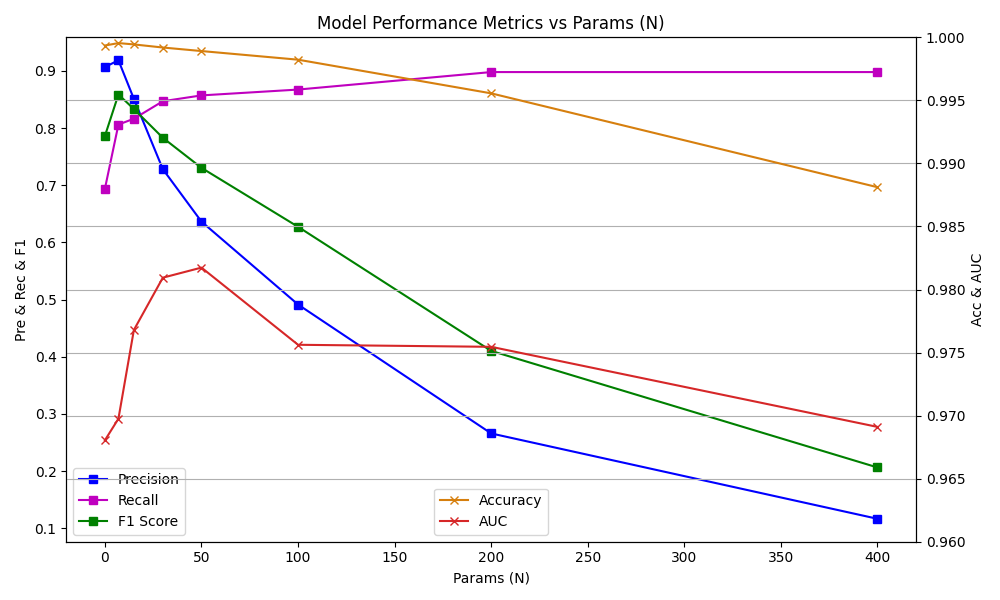
\includegraphics[width=\textwidth]{../Prob1/out/rand_seed_14/task3/Metrics_curve_N_0_7_15_30_50_100_200_400.png}
        \label{fig:Metrics_curve_N_0_7_15_30_50_100_200_400}
        \caption{变化曲线}
    \end{minipage}
\end{figure}
不同典型 N 的ROC曲线
\begin{figure}[H]
    \centering
    \begin{minipage}{0.24\textwidth}
        \centering
        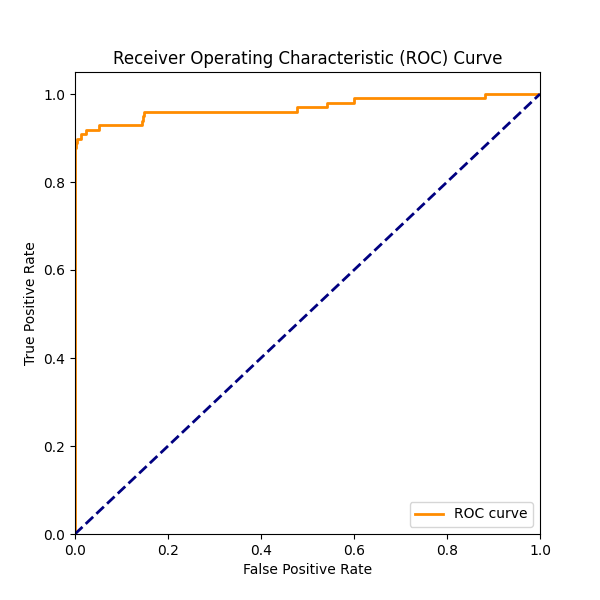
\includegraphics[width=\textwidth]{../Prob1/out/rand_seed_14/task3/roc_curve_N_3_K_7.png}
        \caption{N=3}
        \label{fig:roc_curve_N_3_K_7}
    \end{minipage}
    \begin{minipage}{0.24\textwidth}
        \centering
        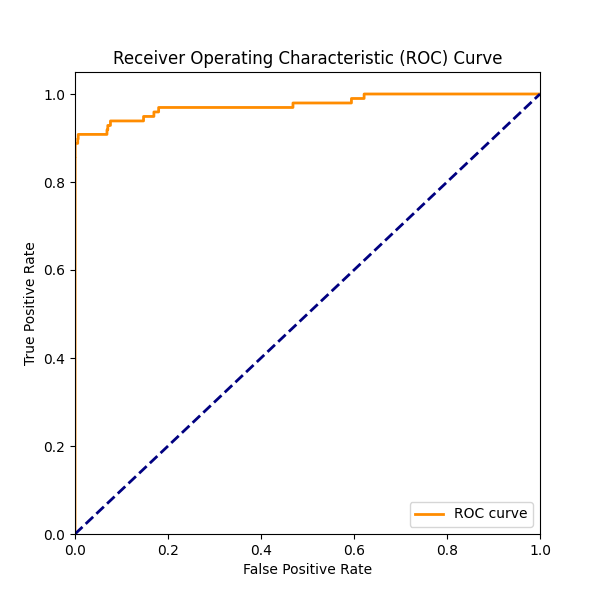
\includegraphics[width=\textwidth]{../Prob1/out/rand_seed_14/task3/roc_curve_N_5_K_7.png}
        \caption{N=5}
        \label{fig:roc_curve_N_5_K_7}
    \end{minipage}
    \begin{minipage}{0.24\textwidth}
        \centering
        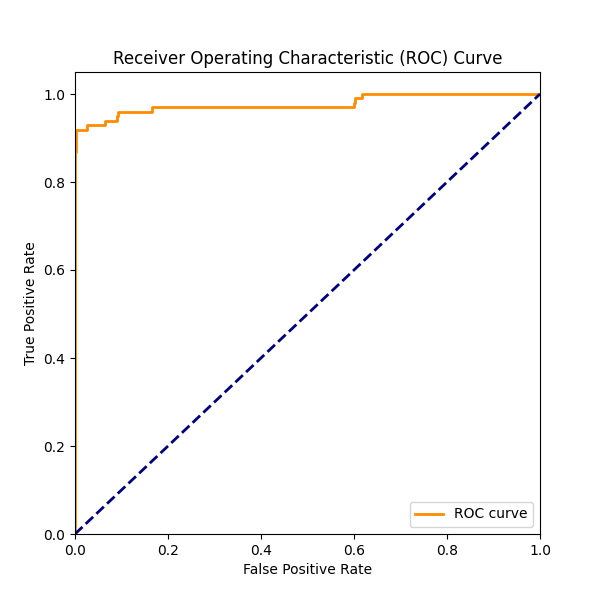
\includegraphics[width=\textwidth]{../Prob1/out/rand_seed_14/task3/roc_curve_N_15_K_7.png}
        \caption{N=15}
        \label{fig:roc_curve_N_15_K_7}
    \end{minipage}
    \begin{minipage}{0.24\textwidth}
        \centering
        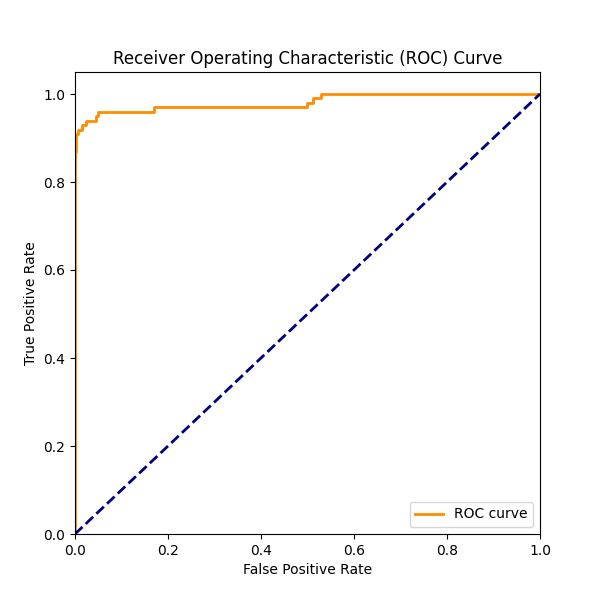
\includegraphics[width=\textwidth]{../Prob1/out/rand_seed_14/task3/roc_curve_N_30_K_7.png}
        \caption{N=30}
        \label{fig:roc_curve_N_30_K_7}
    \end{minipage}
\end{figure}
\begin{figure}[H]
    \centering
    \begin{minipage}{0.31\textwidth}
        \centering
        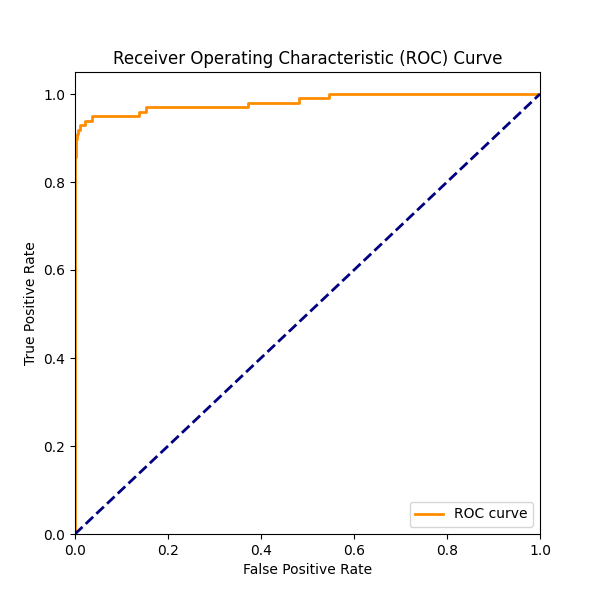
\includegraphics[width=\textwidth]{../Prob1/out/rand_seed_14/task3/roc_curve_N_50_K_7.png}
        \caption{N=50}
        \label{fig:roc_curve_N_50_K_7}
    \end{minipage}
    \begin{minipage}{0.31\textwidth}
        \centering
        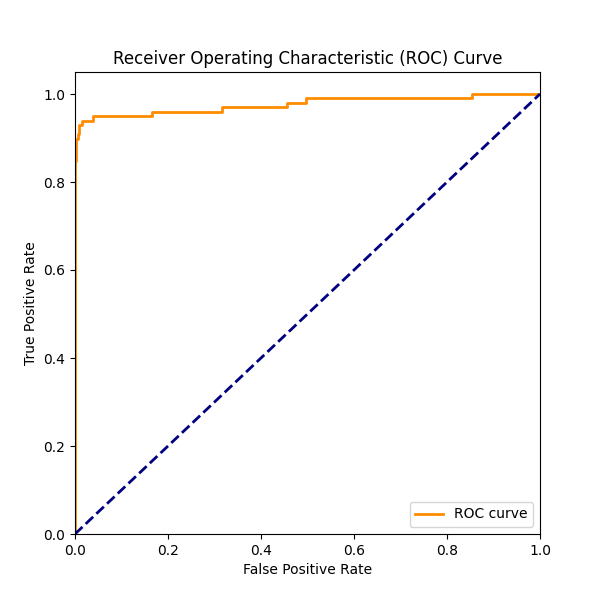
\includegraphics[width=\textwidth]{../Prob1/out/rand_seed_14/task3/roc_curve_N_100_K_7.png}
        \caption{N=100}
        \label{fig:roc_curve_N_100_K_7}
    \end{minipage}
    \begin{minipage}{0.31\textwidth}
        \centering
        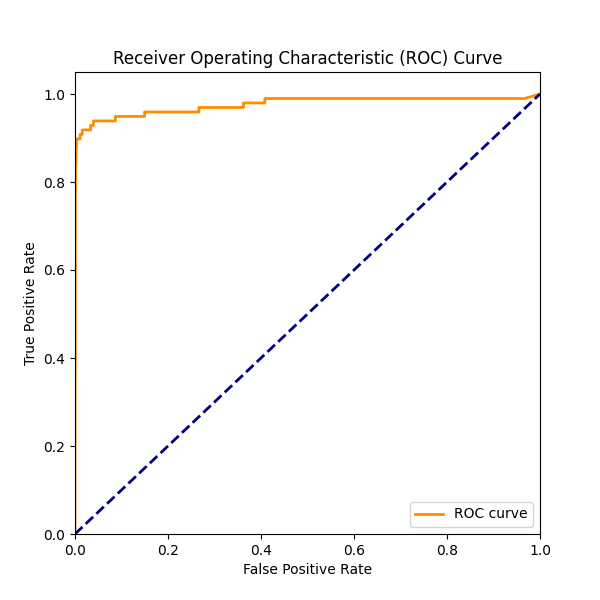
\includegraphics[width=\textwidth]{../Prob1/out/rand_seed_14/task3/roc_curve_N_200_K_7.png}
        \caption{N=200}
        \label{fig:roc_curve_N_200_K_7}
    \end{minipage}
    \begin{minipage}{0.31\textwidth}
        \centering
        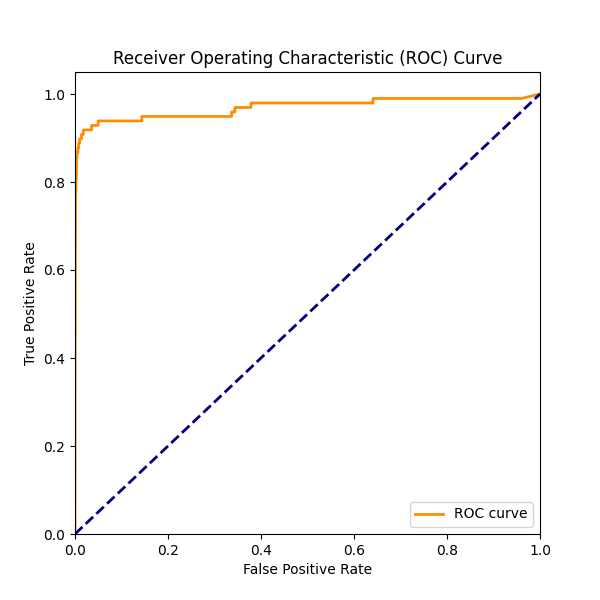
\includegraphics[width=\textwidth]{../Prob1/out/rand_seed_14/task3/roc_curve_N_400_K_7.png}
        \caption{N=400}
        \label{roc_curve_N_400_K_7}
    \end{minipage}
\end{figure}

\subsection*{4.2 结论}
随着 N 的增大,模型的性能逐渐下降,这是因为合成样本的质量下降,过拟合严重,导致模型的泛化能力下降。

缺点:
    \begin{itemize}
        \item 合成样本可能会引入噪声,导致模型过拟合。
        \item 合成样本可能会引入冗余信息,导致模型泛化能力下降。
        \item 合成样本可能会引入错误信息,导致模型性能下降。
        \item 将原本就比较大的训练集变得更大,导致训练时间增加。
    \end{itemize}

\vspace{3em}

\section*{二. (20 points) 机器学习中的过拟合现象}

本题以决策树和多层感知机为例, 探究机器学习中的过拟合现象。 在教材2.1 节中提到, 机器学习希望训练得到的模型在新样本上保持较好的泛化性能. 如果在训练集上将模型训练得“过好”, 捕获到了训练样本中对分类无关紧要的特性, 会导致模型难以泛化到未知样本上, 这种情况称为过拟合。

1.请简要总结决策树和多层感知机的工作原理及其对应的缓解过拟合的手段(决策树相关原理可以参考教材第4 章, 多层感知机可以参考教材第5 章)(5 points);

2.请使用scikit-learn 实现决策树模型, 并扰动决策树的最大深度$max\_ depth$, 一般来说, $max\_ depth$的值越大, 决策树越复杂, 越容易过拟合, 实验并比较测试集精度, 讨论并分析观察到的过拟合现象等(5 points);

3.对决策树算法的未剪枝、预剪枝和后剪枝进行实验比较,并进行适当的统计显著性检验(5 points);

4.请使用PyTorch 或scikit-learn 实现一个简单的多层感知机, 并通过层数、宽度或者优化轮数控制模型复杂度, 实验并比较测试集精度, 讨论并分析观察到的过拟合现象等(5 points)。

注: 请选择1 至 3 个UCI 机器学习库中的数据集进行实验。

\textbf{\large 解:}

\vspace{3em}

\section*{三. (20 points) 激活函数比较}
神经网络隐层使用的激活函数一般与输出层不同. 请画出以下几种常见的隐层激活函数的示意图并计算其导数(导数不存在时可指明), 讨论其优劣(每小题4 points):

\begin{enumerate}
    \item Sigmoid 函数, 定义如下
    \begin{equation}
        f(x) = \frac{1}{1 + e^{-x}}.
        \label{eq:sigmoid}
    \end{equation}
    \item 双曲正切函数 (Hyperbolic Tangent Function, Tanh), 定义如下
    \begin{equation}
        f(x) = \tanh(x) = \frac{e^x - e^{-x}}{e^x + e^{-x}}.
        \label{eq:tanh}
    \end{equation}

    \item 修正线性函数 (Rectified Linear Unit, ReLU) 是近年来最为常用的隐层激活函数之一, 其定义如下
    \begin{equation}
        f(x) = \begin{cases}
            0, & \text{if } x < 0; \\
            x, & \text{otherwise}.
        \end{cases}
        \label{eq:relu}
    \end{equation}

    \item Softplus 函数, 定义如下
    \begin{equation}
        f(x) = \ln(1 + e^x).
        \label{eq:softplus}
    \end{equation}

    \item Leaky Rectified Linear Unit (Leaky ReLU) 函数, 定义如下
    \begin{equation}
        f(x) = \begin{cases}
            \alpha x, & \text{if } x < 0; \\
            x, & \text{otherwise}.
        \end{cases}
        \label{eq:leaky_relu}
    \end{equation}
    其中 $\alpha$ 为一个较小的正数, 比如 0.01.
\end{enumerate}

\textbf{\large 解:}

\vspace{3em}

\section*{四. (30 points) 神经网络实战}
moons是一个简单的二分类数据集,请实现一个简单的全连接神经网络,并参考教材图5.8实现反向传播算法训练该网络,用于解决二分类问题。
\begin{enumerate}
    \item 使用 NumPy 手动实现神经网络和反向传播算法。(15 points)
    \item 实现并比较不同的权重初始化方法。(5 points)
    \item 在提供的moons数据集上训练网络,观察并分析收敛情况和训练过程。(10 points)
\end{enumerate}

\textbf{提示:}

\begin{enumerate}
    \item 神经网络实现:
\begin{itemize}
    \item 实现一个具有一个隐藏层的全连接神经网络。
    \item 网络结构:输入层(2节点) $\rightarrow$ 隐藏层(4节点) $\rightarrow$ 输出层(1节点)
    \item 隐藏层使用 ReLU 激活函数,输出层使用 Sigmoid 激活函数。
    \item 使用交叉熵损失函数。
\end{itemize}
    \item 权重初始化方法。实现以下三种初始化方法,并比较它们的性能:
\begin{itemize}
    \item 随机初始化:从均匀分布 $U(-0.5, 0.5)$ 中采样。
    \item Xavier 初始化:根据前一层的节点数进行缩放。
    \[ W_{ij} \sim U\left( -\frac{\sqrt{6}}{\sqrt{n_{in} + n_{out}}}, \frac{\sqrt{6}}{\sqrt{n_{in} + n_{out}}} \right) \]

其中 \(n_{in}\) 是前一层的节点数,\(n_{out}\) 是当前层的节点数。
    \item He 初始化:He 初始化假设每一层都是线性的,并且考虑了ReLU激活函数的特性。\[ W_{ij} \sim N\left( 0, \frac{2}{n_{in}} \right) \]

其中 \(n_{in}\) 是前一层的节点数。
\end{itemize}
    \item 训练和分析:
\begin{itemize}
    \item 使用提供的 moons 数据集。
    \item 实现小批量梯度下降算法。
    \item 记录并绘制训练过程中的损失值和准确率,训练结束后绘制决策边界。
    \item 比较不同初始化方法对训练过程和最终性能的影响并给出合理解释。
    \item 尝试不同的学习率,观察其对训练的影响并给出合理解释。
\end{itemize}
\end{enumerate}


\textbf{\large 解:}
\begin{lstlisting}[breaklines=true, language=Python, caption=代码实现模板]
"""
注意:
1. 这个框架提供了基本的结构,您需要完成所有标记为 'pass' 的函数。
2. 确保正确实现前向传播、反向传播和梯度更新。
3. 在比较不同初始化方法时,保持其他超参数不变。
4. 记得处理数值稳定性问题,例如在计算对数时避免除以零。
5. 尝试使用不同的学习率(例如 0.01, 0.1, 1),并比较结果。
6. 在报告中详细讨论您的观察结果和任何有趣的发现。
"""
import numpy as np
import matplotlib.pyplot as plt
from sklearn.datasets import make_moons
from sklearn.model_selection import train_test_split

# 生成数据集
X, y = make_moons(n_samples=1000, noise=0.1, random_state=42)
X_train, X_test, y_train, y_test = train_test_split(X, y, test_size=0.2, random_state=42)

class NeuralNetwork:
    def __init__(self, input_size, hidden_size, output_size, init_method='random'):
        self.input_size = input_size
        self.hidden_size = hidden_size
        self.output_size = output_size
        
        # 初始化权重和偏置
        if init_method == 'random':
            # 实现Random初始化
            pass
        elif init_method == 'xavier':
            # 实现Xavier初始化
            pass
        elif init_method == 'he':
            # 实现He初始化
            pass
        else:
            raise ValueError("Unsupported initialization method")

    def relu(self, x):
        return np.maximum(0, x)

    def sigmoid(self, x):
        return 1 / (1 + np.exp(-x))

    def forward(self, X):
        # 实现前向传播
        pass

    def backward(self, X, y, y_pred):
        # 实现反向传播
        pass

    def train(self, X, y, learning_rate, epochs, batch_size):
        # 实现小批量梯度下降训练
        pass

# 辅助函数
def plot_decision_boundary(model, X, y):
    # 绘制决策边界
    pass

def plot_training_process(losses, accuracies):
    # 绘制训练过程
    pass

# 主函数
def main():
    # 创建并训练模型
    # 绘制结果
    pass

if __name__ == "__main__":
    main()
\end{lstlisting}

\end{document}
